% Put some results here

\begin{tcolorbox}
    \begin{center}
        Intelligibility during training
    \end{center}	

\end{tcolorbox}
	 	 %\textsuperscript{[2]}test\par
\begin{center}
	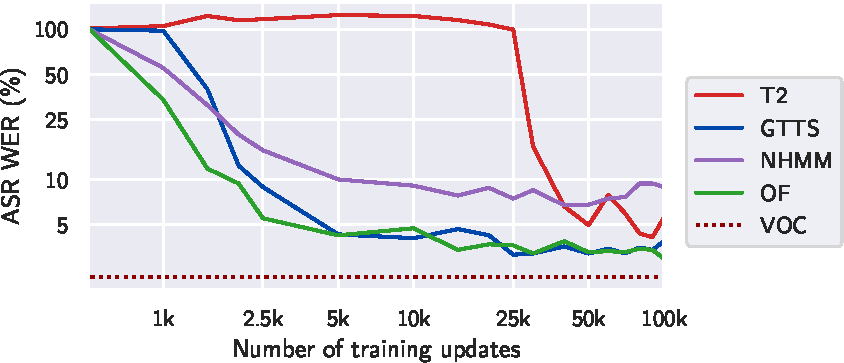
\includegraphics[width=.9\linewidth]{asr_wer.pdf}
\end{center}
Here, we plot the Word Error Rate (WER) of the synthesised utterances using the test set's synthesised utterances during the training course. We plot our proposed system OverFlow (OF) with baseline methods namely, Tacotron 2 (T2), Glow-TTS (GTTS), Neural-HMM\textsuperscript{[3]}, along with the vocoded speech (VOC). Our model converges faster to a lower WER than all the other baselines.

\vspace{1.5em}

\begin{tcolorbox}
    \begin{center}
        Subjective listening test
    \end{center}
\end{tcolorbox}

\begin{center}
	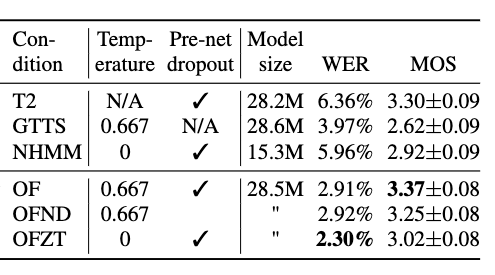
\includegraphics[width=.9\linewidth]{results_table.png}
\end{center}
In a subjective listening test, our method (OF) performs the best compared to other systems while being statistically comparable to T2. Other OF conditions, OFND: OverFlow with No Dropout in prenet and OFZT: OverFlow with Zero Temperature perform fairly in the listening test. Further, we resynthesised the 720 Harvard sentences [32], which are ideal for evaluating intelligibility since they are phonetically balanced. All OverFlow conditions perform substantially better than all baselines on these simple out-of-domain sentences.
\par
\vspace{1.5em}
\par
% \begin{tikzpicture}
% 	\node[anchor=west] at (0,0) {
% 		\begin{minipage}{0.2\textwidth}
% 		\centering
% 		\resizebox{\textwidth}{!}{\includegraphics{homer_smart}}
% 		\end{minipage}
% 	};
% 	\node[anchor=east] at (\textwidth,0) {
% 		\begin{minipage}{0.7\textwidth}
% 		\begin{tcolorbox}
% Test \textsuperscript{[3]}.
% 		\end{tcolorbox}
% 		\end{minipage}
% 	};
% \end{tikzpicture}
% \vspace{1.5em}
% \begin{tcolorbox}
% 	test4
% \end{tcolorbox}

